\chapter{\IfLanguageName{dutch}{Stand van zaken}{State of the art}}%
\label{ch:stand-van-zaken}
% Tip: Begin elk hoofdstuk met een paragraaf inleiding die beschrijft hoe
% dit hoofdstuk past binnen het geheel van de bachelorproef. Geef in het
% bijzonder aan wat de link is met het vorige en volgende hoofdstuk.

% Pas na deze inleidende paragraaf komt de eerste sectiehoofding.

In dit onderdeel wordt alle informatie over de gekende literatuur over dit onderwerp aangekaart. Het is noodzakelijk om een duidelijke kijk te hebben op deze aspecten om de proef goed te begrijpen en succesvol uit te voeren. 

\section{Wat is DevOps}
Het is belangrijk om te weten wat DevSecOps inhoudt voor we hier dieper op in kunnen gaan. Voor we DevSecOps kunnen uitleggen, moeten we weten wat DevOps is. Volgens Microsoft azure kan DevOps gedefinieerd worden als volgt. DevOps, een combinatie van ontwikkeling (Dev) en bedrijfsactiviteiten (Ops), is de bundeling van mensen, processen en technologie om doorlopend waarde aan klanten te bieden \autocite{Azure}. In een DevOps cultuur zullen softwareontwikkeling en IT-operations teams dus samenwerken om betere en betrouwbare producten te maken wat leidt tot hogere prestaties, snellere innovatie en in het algemeen een grotere klanttevredenheid. DevOps richt zich op de volledige levenscyclus van een product, van planning tot levering. Dit wordt ook wel de software development lifecycle (SDLC) genoemd. belangrijk om te weten voor het verdere verloop van deze proef is wat deze levenscyclus inhoudt. Zoals eerder al vermeld begint de cyclus bij een planningsfase. In deze fase werken DevOps-teams aan het ontwikkelen van ideeën en het definiëren van mogelijkheden en functies voor de toepassingen die ze zullen bouwen. De voortgang wordt bijgehouden op verschillende niveaus, van individuele taken voor één enkel product tot een breder arsenaal voor verschillende producten. flexibiliteit en zichtbaarheid plannen in het werk is belangrijk om effectief samen te kunnen werken en waarde te leveren aan klanten. Na de planningsfase komt de ontwikkelingsfase. Deze fase omvat alle technische aspecten van het schrijven van code tot het bouwen van deze code. Er wordt gestreefd naar snelle innovatie zonder onder te doen aan de kwaliteit, stabiliteit en productiviteit. Daarom zullen DevOps-teams focussen op continue integratie en het gebruik van geautomatiseerde testen om te helpen bij een iteratieve ontwikkeling. De volgende fase focust zich op het aanbieden van producten. Het proces van testen, goedkeuren en installeren wordt beschouwd als de levering van een product. De software of update wordt officieel geïmplementeerd bij de eindgebruiker. Hier zullen de teams zowel handmatige stappen ondergaan om alles te controleren als geautomatiseerde systemen laten draaien om alles snel en betrouwbaar te doen. De laatste fase is de operationele fase of het uitvoeren. DevOps-teams houden zich bezig met het onderhouden en monitoren van toepassingen die al in productie zijn. Er wordt ervoor gezorgd dat alles soepel blijft werken en dat eventuele problemen snel worden opgelost. Om te streven naar een hoge beschikbaarheid en systeembetrouwbaarheid zal de toepassing in een productieomgeving ten alle tijden beschikbaar moeten zijn voor gebruikers zonder onverwachte uitvaltijden. Dit zal gerealiseerd worden door problemen proberen te identificeren voor de gebruiker hier last van heeft. Indien dit niet kan geïdentificeerd worden op voorhand zullen ze de impact minimaliseren door problemen op tijd op te lossen. 

\section{Wat is DevSecOps}

DevSecOps staat voor Development Security en Operations. In tegenstelling tot DevOps zal er bij DevSecOps een belangrijke rol zijn voor security in de volledige levenscyclus. Vroeger was een IT-security team afgesloten van het proces en waren ze enkel belangrijk aan het einde van het proces. Dit was een aantal jaren geleden geen probleem aangezien ontwikkelingscyclussen maanden tot jaren konden duren. Een goede DevOps gang van werken die op dit moment aan de orde is, heeft meer nood aan het integreren van security doorheen de cyclus aangezien er nood is aan continue integratie. DevSecOps wil zeggen dat er moet nagedacht worden over zowel applicatie als infrastructurele beveiliging vanaf het begin tot het einde \autocite{RedHat2023}. \ref{fig:linear} 

\begin{figure}[h]
    \centering
    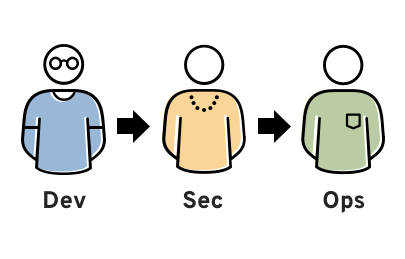
\includegraphics{devsecops-linear.png}
    \caption{lineaire weergeving DevSecOps} \autocite{RedHat2023}
    \label{fig:linear}
\end{figure}

\section{Verschillende automatisatie tools}
DevSecOps heeft nood aan verschillende tools om aan goede continue levering en continue integratie (CI/CD) te doen. Automatisatie is sleutelstuk in de moderne development pijplijn en helpt DevSecOps teams met beveiliging doorheen alle development fasen zonder de pijplijn te vertragen. Er zijn drie belangrijke doelen voor DevSecOps tools. Allereerst is het belangrijk om de kans op risico's te vermijden zonder de snelheid te beïnvloeden. Dit wordt bereikt door continue beveiligingstesten te implementeren. Deze helpen om zwakheden in de beveiliging te herstellen. Een tweede belangrijk doel is om beveiligingsteams te ondersteunen bij automatisatie. Dit helpt om ontwikkelingsprojecten niet manueel te moeten bekijken na elke release. Als laatste is het belangrijk om beveiliging naar links te schakelen in de software development lifecycle om beveiliging sneller te implementeren in het proces.\autocite{Tigera2024}

\subsection{codeAI}




